
\section{Simulations}\label{sec:exp}

In this section, we present simulations to complement our theoretical results.
In the first experiment, we show that the generalization performance of gradient descent depends on the choice of initialization.
In particular, smaller initializations enjoy better generalization performance than larger initializations.
In the second experiment, we demonstrate that gradient descent can run for a large number of  iterations and the test error keeps decreasing, which suggests early stopping is not necessary. 
In the third experiment, we show that a natural projected gradient descent procedure works poorly compared to gradient descent on the factorized model, which suggests the power of using a factorized model.
In the last experiment, we report results for running stochastic gradient descent on the quadratic neural network setting, starting from a large initialization.

We generate the true matrix by sampling each entry of $\bUg$ independently from a standard Gaussian distribution and let $\bXg = \bUg \bUg^\top$. 
Each column of $\bUg$ is normalized to have unit norm, so that the spectral norm of $\bXg$ is close to one.
For every sensing matrix $A_i$, for $i = 1,\dots,m$, we sample the entries of $A_i$ independently from a standard Gaussian distribution.
Then we observe $b_i = \innerProduct{A_i}{\bXg}$.
When an algorithm returns a solution $\hat X$, we measure training error by:
\[ \sqrt{\frac{\sum_{i=1}^m (\innerProduct{A_i}{\hat X} - b_i)^2} {\sum_{i=1}^m b_i^2}.} \]
We measure test error by:
\[ \frac{\normFro{\hat X - \bXg}} {\normFro{\bXg}}. \]
For the same $\bXg$, we repeat the experiment three times, by resampling the set of sensing matrices $\{A_i\}_{i=1}^m$.
We report the mean and the error bar.

\paragraph{Choice of initialization.}
Let $U_0 = \alpha \Id$.
We use $m = 5dr$ samples, where rank $r = 5$.
We plot the training and test error for different values of $\alpha$.
Figure \ref{fig_init} shows that the gap between the training and test error
narrows down as $\alpha$ decreases.
We use step size $0.0025$ and run gradient descent for $10^4$ iterations.

\begin{figure}[!ht]
	\centering
	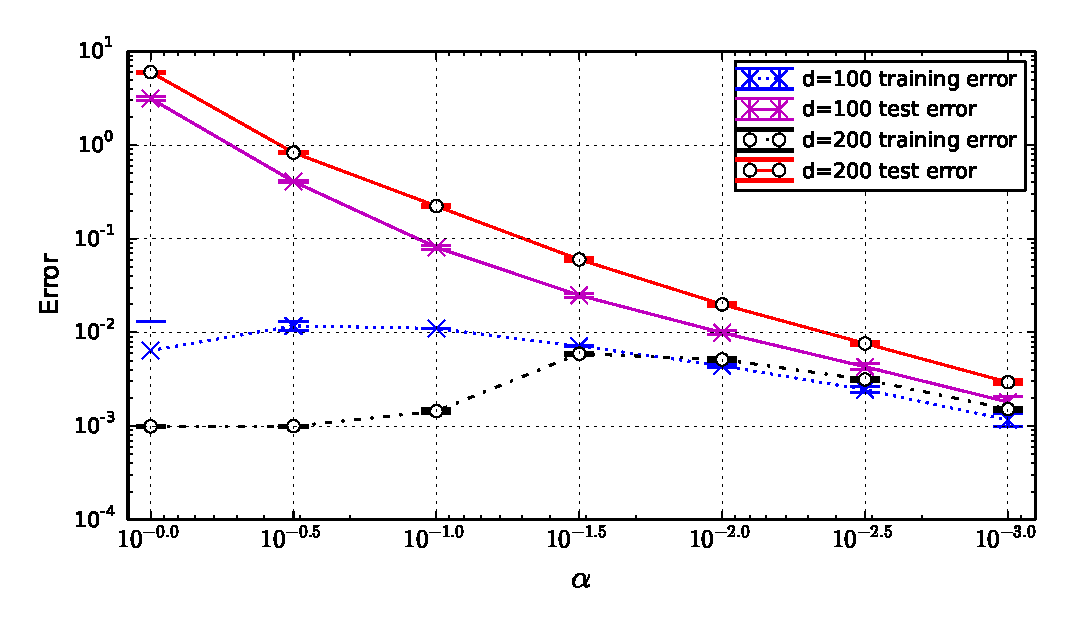
\includegraphics[width=0.5\textwidth]{compare_init.eps}
	\caption{Generalization performance depends on the choice of initialization:
	the gap between training and test error decreases as $\alpha$ decreases.
	Here the number of samples is $5dr$, where rank $r = 5$. We initialize with
	$\alpha \Id$, and run $10^4$ iterations with step size $0.0025$.}
	\label{fig_init}
\end{figure}

In Figure \ref{fig_init_long}, we run for longer iterations to further compare the generalization performance of initialization $U_0 = \alpha\Id$ for $\alpha = 1.0, 10^{-3}$.
We report the mean values at each iteration over three runs.
When $\alpha = 1.0$, despite the training error decreases below $10^{-4}$,
the test error remains to be on the order of $10^{-1}$.

\begin{figure}[!ht]
	\centering
	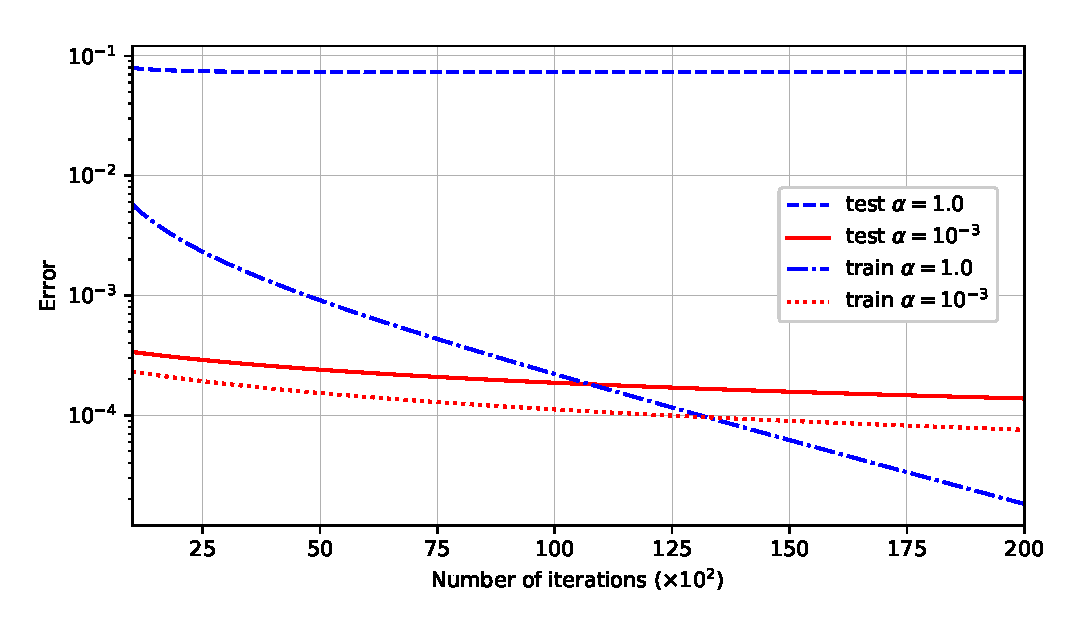
\includegraphics[width=0.5\textwidth]{compare_init_long_step.eps}
	\caption{Further comparison between the generalization performance of large versus small initializations. We plot the data points from iteration 500 onwards to simplify the scale of the y-axis. The step size is $0.0025$.}
	\label{fig_init_long}
\end{figure}



\paragraph{Accuracy.}
In this experiment, we fix the initialization to be $U_0 = 0.01 \Id$,
and apply the same set of parameters as the first experiment.
We keep gradient descent running for $10^5$ iterations, to see if test error
keeps decreasing or diverges at some point.
Figure \ref{fig_accuracy} confirms that test error goes down gradually.
%It would be interesting to understand whether the same observation holds when
%the sensing matrices satisfy restricted isometry property more generally --- we leave it to future work.

\begin{figure}[!ht]
	\centering
	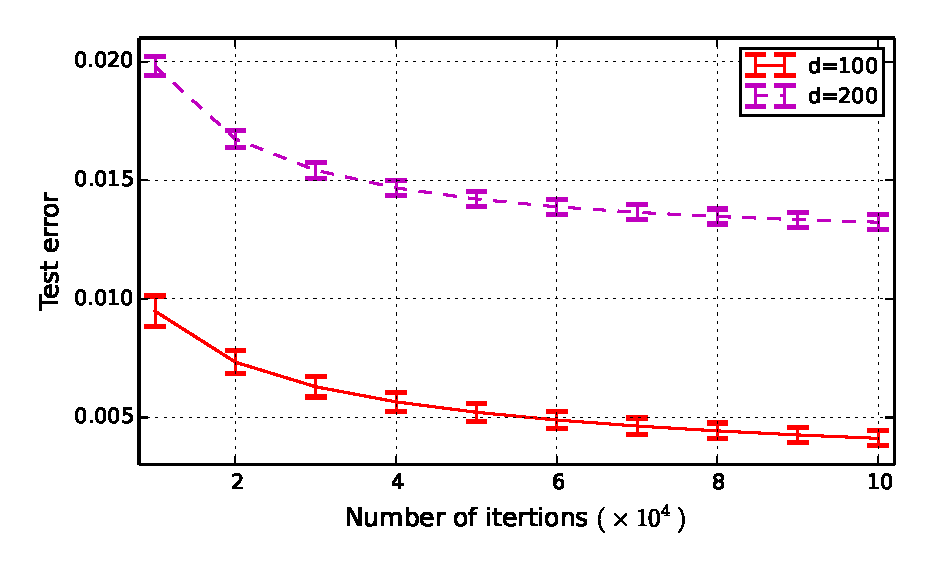
\includegraphics[width=0.5\textwidth]{accuracy.eps}
	\caption{Test error keeps decreasing as the number of iterations goes to $10^5$. Here the number of samples is $m = 5dr$, where rank $r = 5$. Note that the initial test error is approximately $1$.}
	\label{fig_accuracy}
\end{figure}

\paragraph{Projected gradient descent.}
In this experiment, we consider the following natural projected gradient descent (PDG) procedure.
Let $f(X) = \frac 1 m \sum_{i=1}^m \left(\innerProduct{A_i}{X} - b_i \right)^2$.
At every iteration, we first take a gradient step over $f(X)$,
then project back to the PSD cone.
We consider the sample complexity of PGD by varying the number of sensing
matrices $m$ from $5d$ to $35d$.
Here the rank of $\bXg$ is $1$.
We found that the performance of PGD is much worse compared to gradient descent on the factorized model.
For both procedures, we use step size equal to $0.0025$.
We stop when the training error is less than $0.001$, or when the number of iterations reaches $10^4$.
Figure \ref{fig_pgd} shows that gradient descent on the factorized model
consistently recovers $\bXg$ accurately.
On the other hand, the performance of projected gradient descent gets even worse as $d$ increases from $100$ to $150$.

\begin{figure}[!ht]
	\centering
	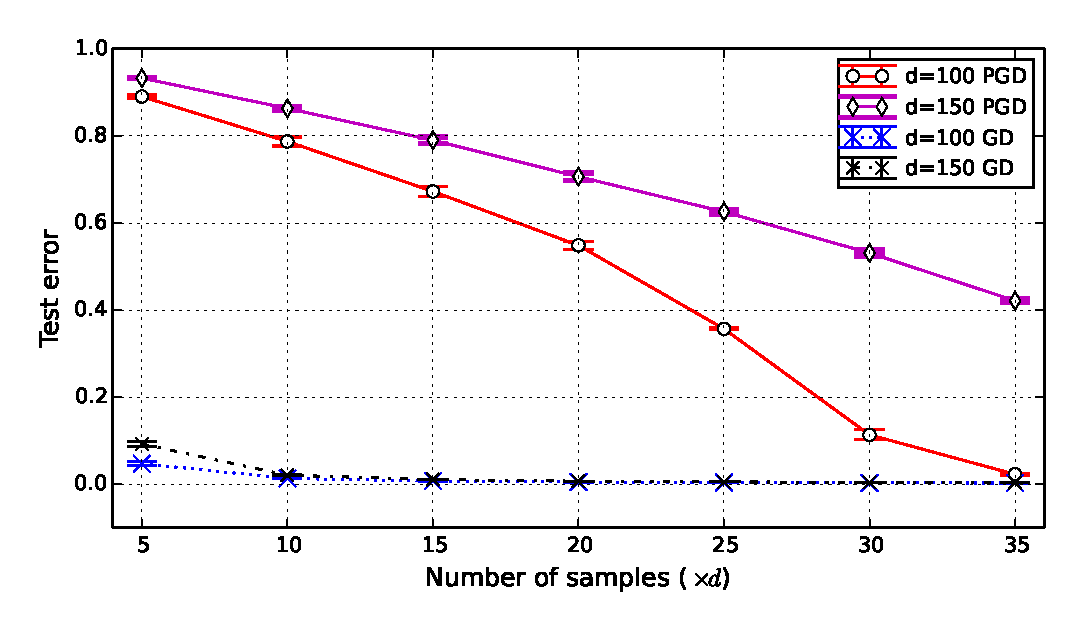
\includegraphics[width=0.5\textwidth]{compare_PGD.eps}
	\caption{Projected gradient descent (PGD) requires more samples to recover $\bXg$ accurately,
	than gradient descent on the factorized model.
	Moreover, the performance of PGD gets worse as $d$ increases.}
	\label{fig_pgd}
\end{figure}

\paragraph{Stochastic gradient descent.}
In this experiment, we complement our theoretical results by running stochastic gradient descent from large initializations.
We generate $m = 5dr$ random samples and compute their true labels as the training dataset.
For stochastic gradient descent, at every iteration we pick a training data point uniformly at random from the training dataset.
We run one gradient descent step using the training data point.
We initialize with $U_0 = \Id$ and use step size $8 \times 10^{-5}$.
Figure \ref{fig_sgd} shows that despite the training error decreases to $10^{-7}$, the test error remains large.
We also report the results of running gradient descent on the same instance for comparison.
As we have already seen, Figure \ref{fig_gd_quadratic} shows that gradient descent also gets stuck at a point with large test error, despite the training error being less than $10^{-7}$.


\begin{figure}[!ht]
	\centering
	\subfigure[Stochastic gradient descent]%
	{\label{fig_sgd}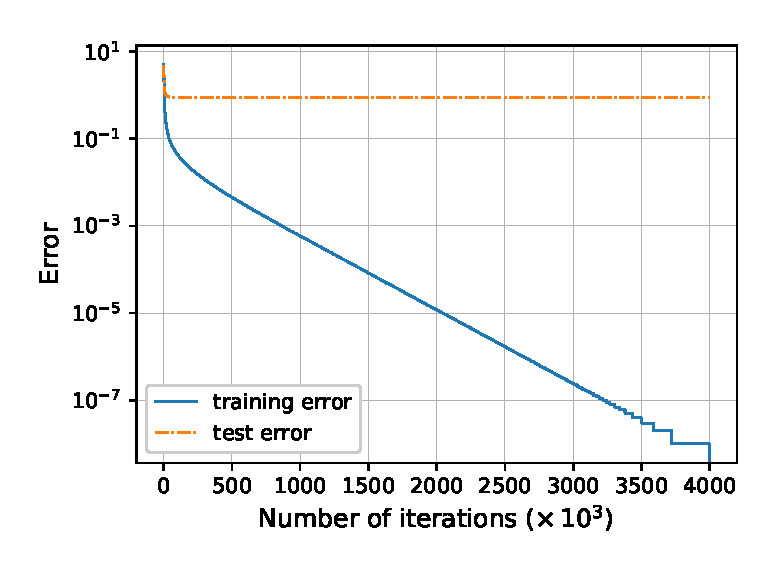
\includegraphics[width=.45\linewidth]{sgd_matrix.eps}}
	\subfigure[Gradient descent]%
	{\label{fig_gd_quadratic}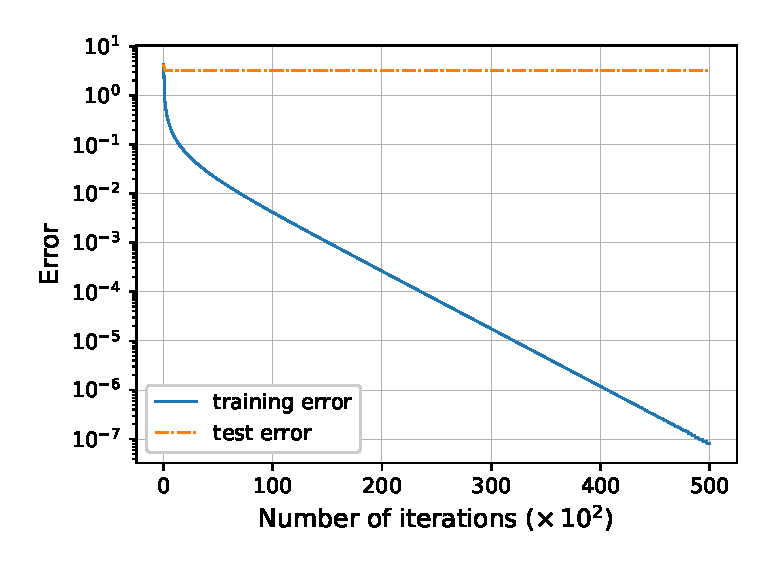
\includegraphics[width=.45\linewidth]{gd_matrix.eps}}
	\caption{Stochastic gradient descent, when initialized with the identity matrix, does not generalize to test data. Here $d = 100$ and $r = 5$.}
\end{figure}

